\documentclass[slide05.tex]{subfiles}
\begin{document}
\begin{frame}[plain]
    \begin{center}
        \vspace{48pt}
        {\huge\bf センサーについて知ろう}
    \end{center}
\end{frame}

\begin{frame}
    \frametitle{ボタン}
    \begin{center}
        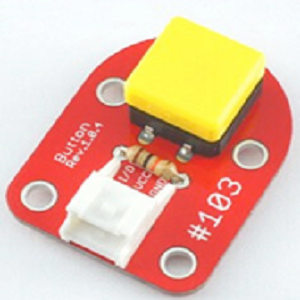
\includegraphics[width=0.4\textwidth]{../../asset/image/text05-img028.png}
        \begin{itemize}
            \item ボタンが押されている間、値が1
            \item ボタンが押されていないと値が0
        \end{itemize}
    \end{center}
    \textpageref{9}
\end{frame}

\begin{frame}
    \frametitle{傾斜センサ}
    \begin{center}
        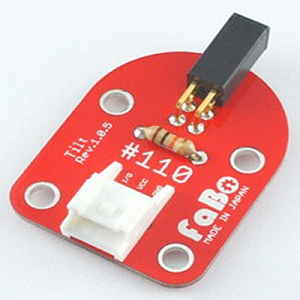
\includegraphics[width=0.4\textwidth]{../../asset/image/text05-img018.png}
        \begin{itemize}
            \item 傾いているかどうかがわかる
            \item 黒い部分の中にたまが入っていて、かたむくと値が変わる
            \item 使用例：ストーブの安全装置
        \end{itemize}
    \end{center}
    \textpageref{9}
\end{frame}

\begin{frame}
    \frametitle{スイッチ}
    \begin{center}
        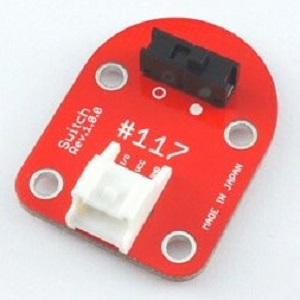
\includegraphics[width=0.4\textwidth]{../../asset/image/text05-img019.jpg}
        \begin{itemize}
            \item スイッチがオンのとき値が1になる
            \item スイッチがオフのとき値が0になる
            \item オンのまま、オフのままにできる
        \end{itemize}
    \end{center}
    \textpageref{10}
\end{frame}

\begin{frame}
    \frametitle{リミットスイッチ}
    \begin{center}
        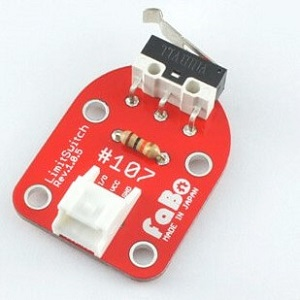
\includegraphics[width=0.4\textwidth]{../../asset/image/text05-img020.jpg}
        \begin{itemize}
            \item スイッチが押されたとき値が1になる
            \item スイッチが押されていないとき値が0になる
            \item 例：ふたがしまったかどうか
        \end{itemize}
    \end{center}
    \textpageref{10}
\end{frame}

\begin{frame}
    \frametitle{センサーをピンにつけてみよう}
    \begin{center}
        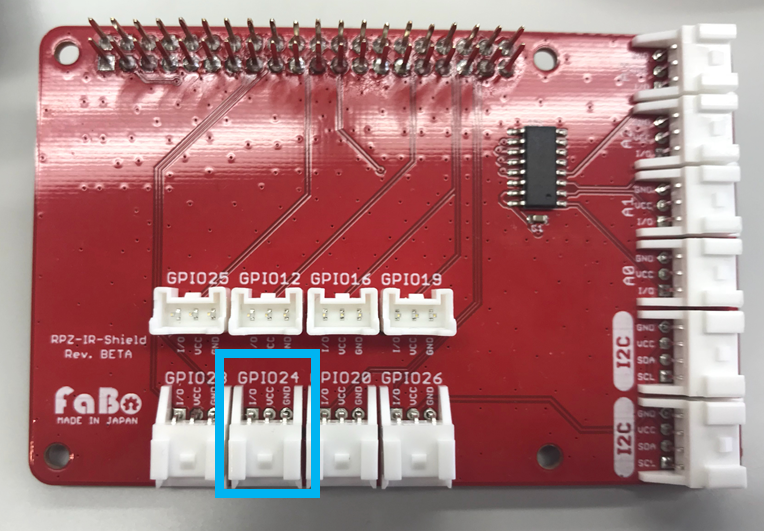
\includegraphics[width=0.7\textwidth]{../../asset/image/text05-img029.png}
        \begin{itemize}
            \item GPIO23とLEDをつなげてみよう
            \item GPIO24と入力センサをつなげてみよう
            \item HSPで\textasciitilde/05/digin.hspを動かしてみよう
        \end{itemize}
    \end{center}
    \textpageref{14}
\end{frame}

\begin{frame}[fragile]
    \frametitle{デジタル入力センサを使った\\プログラム}
    \begin{lstlisting}[title=\textasciitilde/05/digin.hsp]
    #include "hsp3dish.as"
    #include "rpz-gpio.as"

    *main
	    redraw 0
	    pos 30,30
	    mes "デジタル入力そうちでLEDを光らせよう"
	    redraw 1
	    if gpioin(24)=1 : goto *digital_on
	    goto *digital_off
        
    *digital_on
	    gpio 23, 1
	    wait 10
	    goto *main

    *digital_off
	    gpio 23, 0
	    wait 10
	    goto *main 
    \end{lstlisting}
    \textpageref{14}
\end{frame}

\begin{frame}[fragile]
    \begin{exampleblock}{問題を解いてみよう}
    \begin{itemize}
        \item 教科書15ページ 問題5-5
        \begin{itemize}
            \item 5問を授業中にやる
        \end{itemize}
        \item 教科書15ページ 問題5-6
        \begin{itemize}
            \item 2問は宿題。時間があったら授業中にやる
        \end{itemize}
    \end{itemize}
    \end{exampleblock}
\end{frame}
\end{document}
